\section{全液压矫直机智能自学习的矫直模型及其电液伺服控制理论}

文献\parencite{zhinengjiaozhiji}所述矫直机是中厚板生产流水线的重要一环,中厚板滚式板材矫直机布置在冷控之后,保证了板材的不平精度、减轻了板材的残余应力的影响,成为轧线上的重要设备之一。

未矫直的中厚板材,送入矫直机后,矫直机的直辊上下布置并在合适的位置给予进给的中厚板一系列辊压力。如果直辊布置的位置处于一个合适的位置,被矫直中厚板将会被较好的矫直。该矫直工艺的技术难点在于如何布置直辊的相对位置。

如图\ref{fig:jiaozhiji},文献\parencite{zhinengjiaozhiji}给出了其研究的位于实验室的全液压矫直机。该矫直机大致由电气系统、液压系统和机械系统组成。

\begin{figure}[!htp]
	\centering
	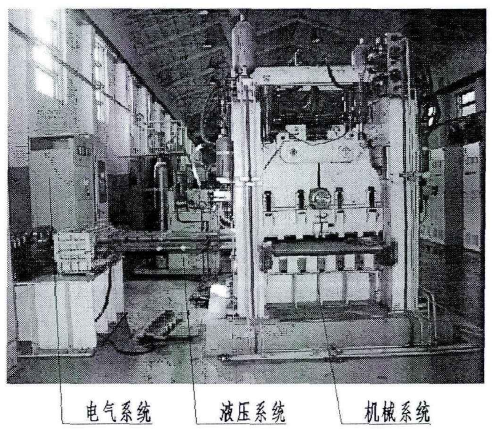
\includegraphics[width=\textwidth]{IMG/jiaozhiji.png}
	\bicaption[实验室全液压矫直机]
		{实验室全液压矫直机}
		{Full hydraulic straightening machine in laboratory}
	\label{fig:jiaozhiji}
\end{figure}

文献\parencite{zhinengjiaozhiji}研究的是一种一种十一辊矫直机,其主要工作部件是由液压系统控制的十一个直辊。

该十一个直辊各有一个以上的自由度,可以由控制机构驱动其轴在竖直面上的相对位置。某个时刻对于指定材料指定尺寸指定工况总存在最佳的直辊相对布置位置的解,如何找到这个最优解是该研究的重点。

控制直辊偏移量的液压缸是一种非对称电液伺服缸,输入的电压信号转换为非对称阀阀芯的偏移量,从而控制非对称缸的工作杆发生位移输出直辊位移形成特定的直辊布置。

\begin{figure}[!htp]
	\centering
	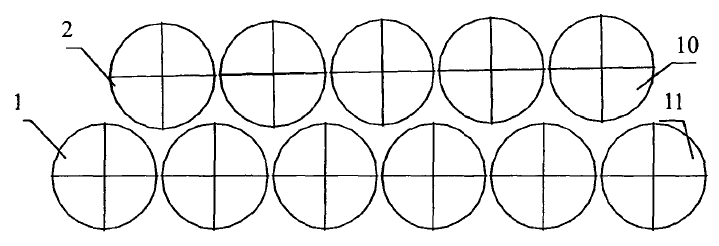
\includegraphics[width=\textwidth]{IMG/shiyigun.png}
	\bicaption[十一辊矫直机直辊布置图]
		{十一辊矫直机直辊布置图}
		{Layout of 11 roller straight roller}
	\label{fig:shiyigun}
\end{figure}

如图\ref{fig:hyserver}给出了控制直辊的电液伺服系统,该系统由电磁伺服阀和工作液压缸组成,将电压信号最终转换为液压缸活塞杆的位移。

如图\ref{fig:hycontrolsys}给出了该伺服系统的闭环控制框图。

\begin{figure}[!htp]
	\centering
	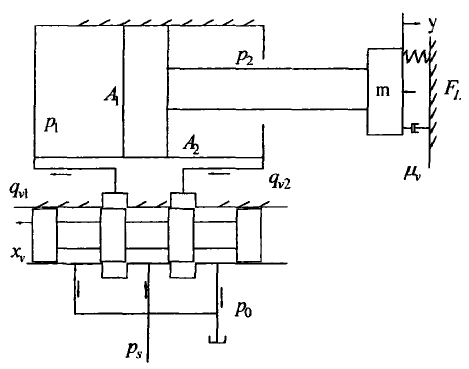
\includegraphics[width=\textwidth]{IMG/hyserver.png}
	\bicaption[全液压矫直机电液伺服系统原理图]
		{全液压矫直机电液伺服系统原理图}
		{Schematic of hydraulic straightener electrohydraulic servo system}
	\label{fig:hyserver}
\end{figure}

\begin{figure}[!htp]
	\centering
	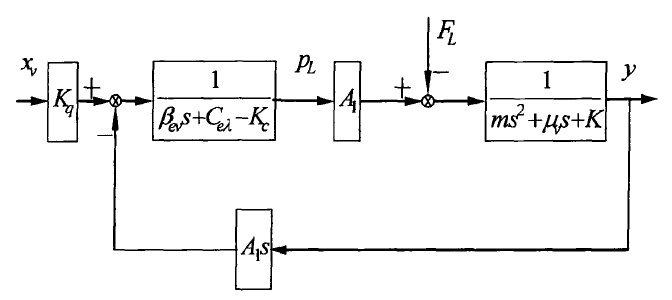
\includegraphics[width=\textwidth]{IMG/hycontrolsys.png}
	\bicaption[非对称阀控制非对称缸系统方框图]
		{非对称阀控制非对称缸系统方框图}
		{Asymmetric valve control asymmetric cylinder system block diagram}
	\label{fig:hycontrolsys}
\end{figure}

如何输入电压信号才能获得较好的矫直质量,这属于控制理论的研究范畴。要获得较好的矫直质量,传统的控制理论如经典PID控制理论的应用在全液压矫直机上比较困难,针对不同设备、产品和工况需要专门的计算分析整定PID控制参数。

文献\parencite{zhinengjiaozhiji}对该液压系统的智能设计体现在下述电液伺服系统控制方案的智能化研究。

如图\ref{fig:netcontrol}给出一种流行的现代控制理论,多控制量的神经元控制器,该控制器是一种神经元网络,能够通过对输入输出结果进行学习和遗传,使矫直机获得较好的控制质量。

\begin{figure}[!htp]
	\centering
	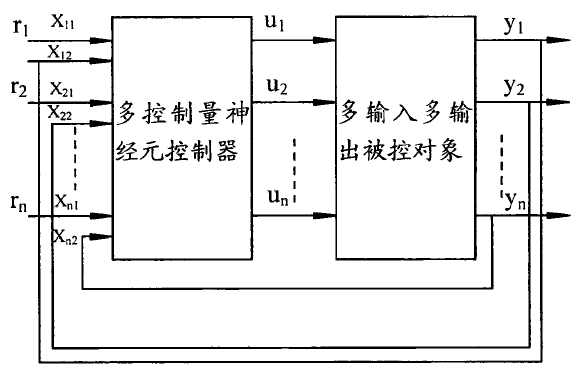
\includegraphics[width=\textwidth]{IMG/netcontrol.png}
	\bicaption[多控制量神经元闭环控制系统]
		{多控制量神经元闭环控制系统}
		{Multi-control neuron's net of closed-loop control system}
	\label{fig:netcontrol}
\end{figure}

如图\ref{fig:fuzzycontrol}给出了另外一种现代控制理论,这是一种模糊控制理论的应用。该控制模型接受模糊量和精确量的输入,通过专家库和模糊规则基支持的模糊推理机的处理,解模糊并输出精确量。

如图\ref{fig:selflearn}给出了较为完整的、研究所述全液压矫直机的总体控制框架。

\begin{figure}[!htp]
	\centering
	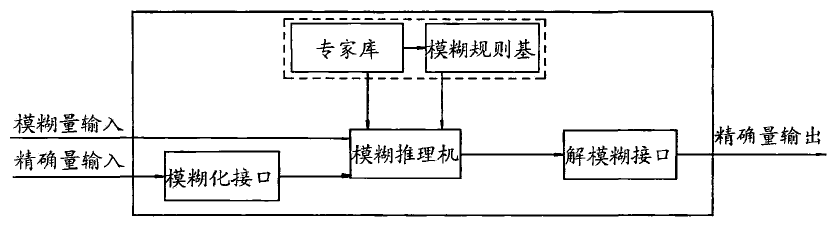
\includegraphics[width=\textwidth]{IMG/fuzzycontrol.png}
	\bicaption[全液压矫直机模糊逻辑系统结构图]
		{全液压矫直机模糊逻辑系统结构图}
		{Hydraulic straightener fuzzy logic system structure diagram}
	\label{fig:fuzzycontrol}
\end{figure}

\begin{figure}[!htp]
	\centering
	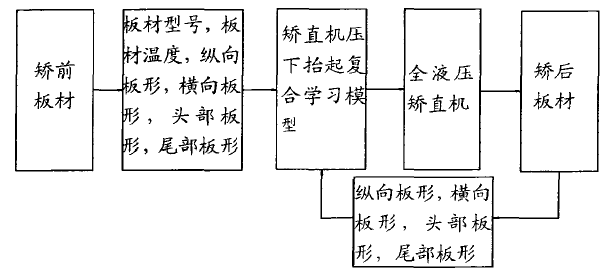
\includegraphics[width=\textwidth]{IMG/selflearn.png}
	\bicaption[全液压矫直机矫直模型自学习系统]
		{全液压矫直机矫直模型自学习系统}
		{Hydraulic straightening machine straightening model self-learning system}
	\label{fig:selflearn}
\end{figure}

文献\parencite{zhinengjiaozhiji}这个例子体现了现代先进控制理论应用在生产设备中,智能地驱动液压系统高质量完成作业。
